\begin{savequote}[75mm]
We have arranged a civilization in which most crucial elements profoundly depend upon science and technology.
\qauthor{Carl Sagan (1934-1996)}
\end{savequote}

\chapter{Introduction}
\label{Introduction}

\newpage

\section{The Energy-Water Nexus}
  
\newthought{Nearly all modern industrialized societies} rely upon energy generation technologies which are derivatives of a thermodynamic process known as the heat engine. In a typical heat engine the chemical energy stored within a fuel source such as coal, petroleum, or natural gas, must be first be released as thermal energy through the process of combustion. During combustion the rapid oxidation of the fuel transforms its stored chemical energy into thermal energy which is then released into the ambient environment as heat. A heat engine is an engineered system which is capable o  converting this ambient thermal energy into mechanical energy for the purpose of performing some sort of work -- i.e. generating electricity. In the majority of heat engines this conversion from thermal to mechanical energy is most efficiently accomplished via the differential heating of a working fluid -- most typically, water.
    
    The history of the evolution of human energy systems is a story of the progressive discovery and expanded exploitation of new, higher density chemical energy stores, and new, higher efficiency mechanical systems for the combustion of chemical fuels or the transformation of thermal to mechanical energy. Nowhere however, in this history however has there occurred a single substantial advance in the choice of the working fluid to be used within the heat engine: water. For all of the advances which have been made in terms of improved fuel processing, boiler and combustion chamber design, water has remained stubbornly positioned as a critical component of nearly all major commercial scale energy systems; but in particular, those involved with the production of electricity. 
    
    In a similar vein, another foundation pillar of industrialized society is the mechanized disposal of human and animal wastes via constructed sewage conveyance and treatment systems. 
    
     \begin{figure}[Perspectives on the \it{Energy-Water Nexus}]
       \centering
       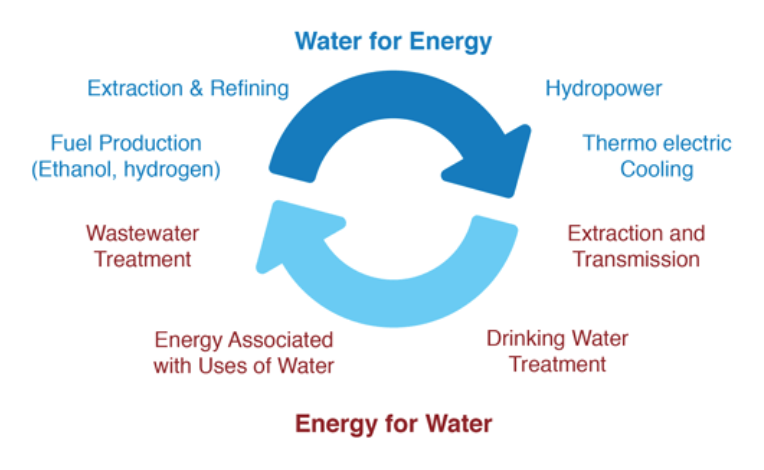
\includegraphics[width=4.5in]{figures/energy-water-nexus-perspectives.png}
       \caption[Perspectives on the \it{Energy-Water Nexus}]{Perspectives on the \it{Energy-Water Nexus}}
       \label{fig:energy-water-perspectives}
     \end{figure}
    
There are two perspectives from which the \textit{Energy-Water Nexus} can be alternatively studied. The first emphasizes the \textit{Water for Energy} dimension, and is generally concerned with the study of processes and technologies that are involved with the direct withdrawal and consumption of water for the production of both primary and final energy resources. The second of these perspectives, and the one which shall be adopted for the purposes of this proposal, focuses instead on the \textit{Energy for Water} dimension; investigating processes and technologies which consume energy for the purpose of transmitting or purifying freshwater resources. 
    
     \begin{figure}[Dimensions of the \it{Energy-Water Nexus}]
       \centering
       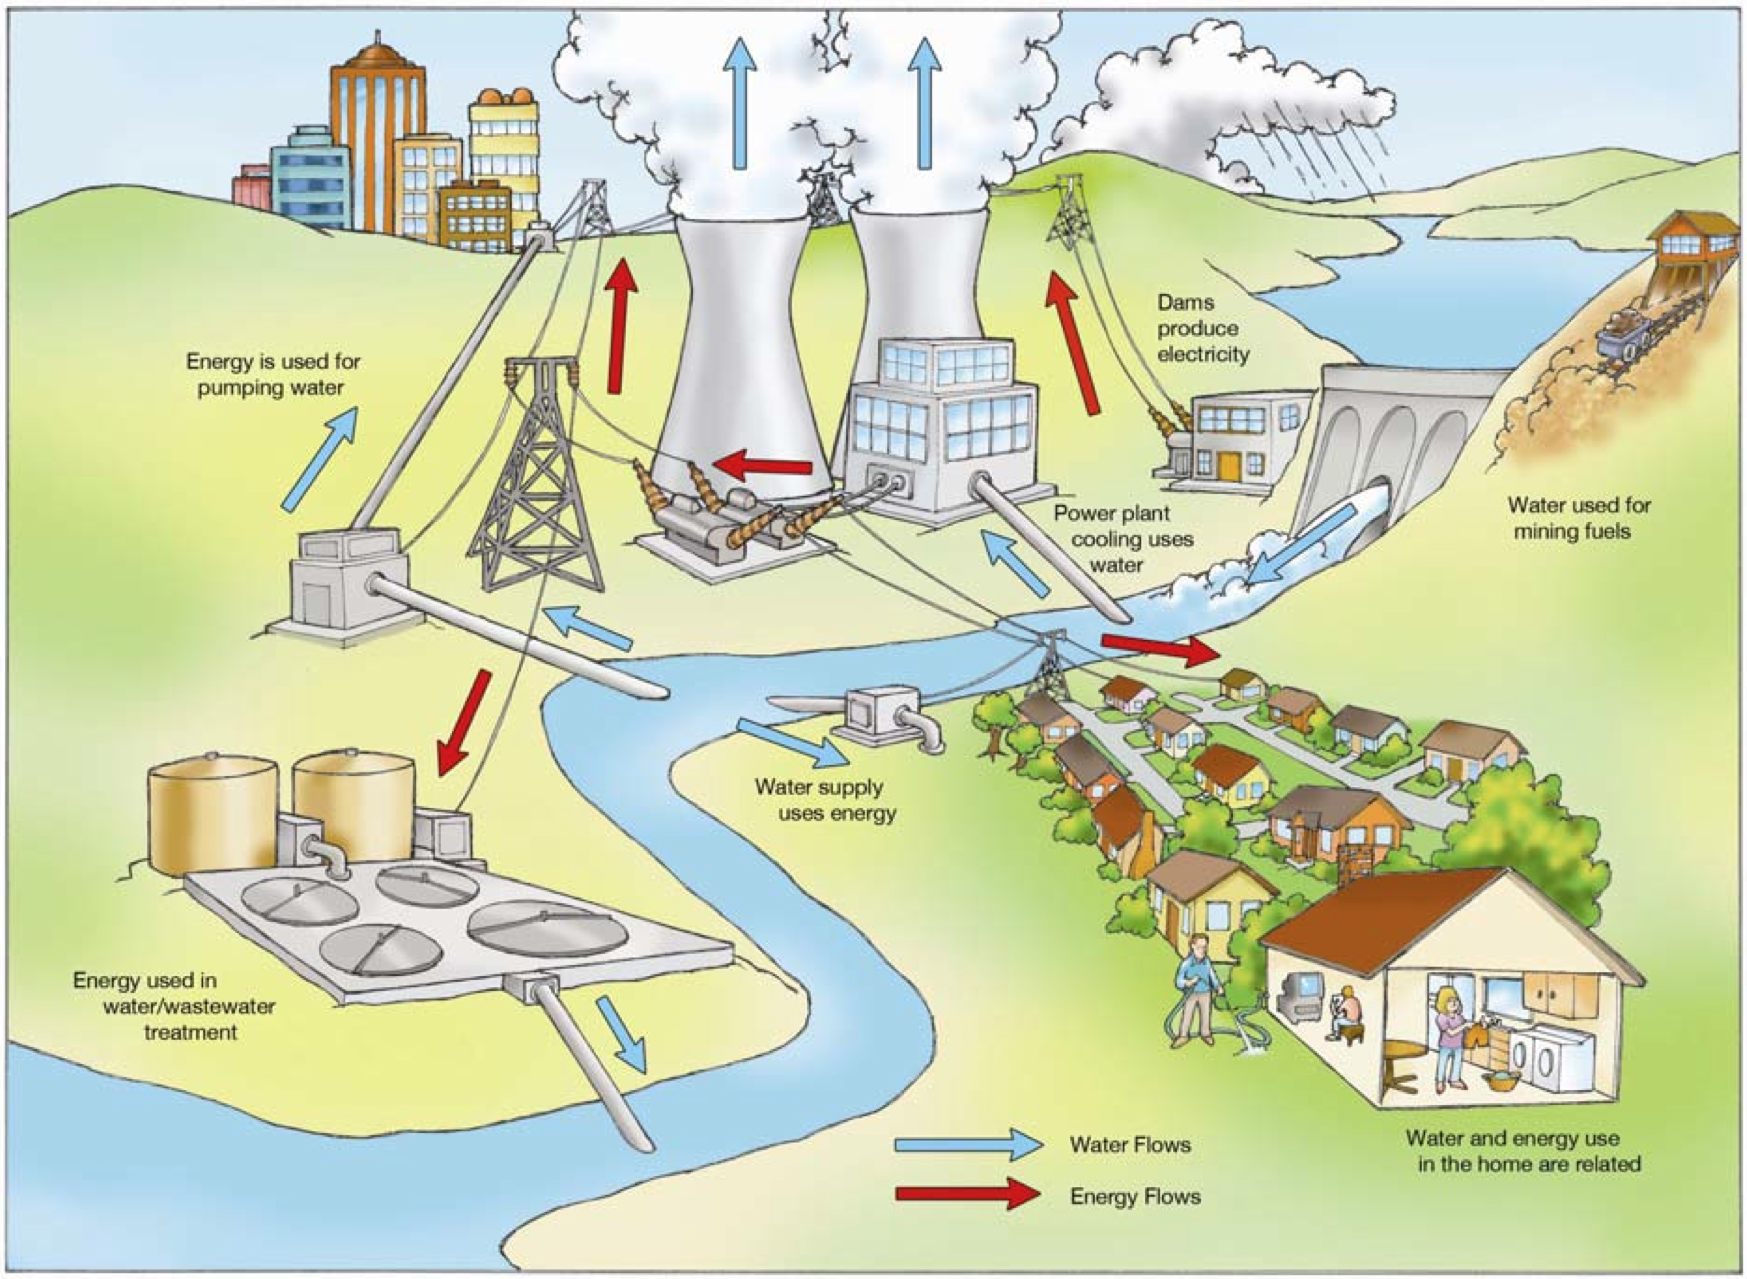
\includegraphics[width=5.5in]{figures/energy-water-nexus-dimensions.png}
       \caption[Dimensions of the \it{Energy-Water Nexus}]{The dimensions of the \it{Energy-Water Nexus}}
       \label{fig:energy-water-dimensions}
     \end{figure}
    
Here in the United States, 50\% of total annual freshwater withdrawals are used for the cooling of thermoelectric power plants. Alternatively, 4\% of the nation's total energy consumption is dedicated to the transmission and purification of water and wastewater. While these national figures speak to the overall significance of this issue, the situation becomes more acute when one begins to consider different regional contexts. 
    
The criticality of the \textit{Energy-Water Nexus} becomes greatly exacerbated in those areas where water availability is scarce (relative to the quantity and distribution of demand) and/or energy prices are high. Unfortunately, the state of California suffers from both of these conditions, making the \textit{Energy-Water Nexus} a frequent source of regional interest within both the academic research a policy communities. For example, in a 2005 report published by the California Energy Commission (CEC) it was found that 19\% of the electricity and 32\% of the natural gas consumed within the entire state were used for purpose directly related to the supply and treatment of freshwater resources.
    
\section{Water Distribution Systems}
    
One of the main drivers for of this tremendous energy consumption within the state of California is the large scale transfer of freshwater resources between distinct hydrologic basins. California is crossed longitudinally by a massive network of interconnected hydraulic engineering projects including pipelines, aqueducts, reservoirs, and pump stations. These systems, which have been funded by a mixture of Federal, State, and Local agencies, were designed to reconcile discontinuities between the spatial and temporal distributions of the supply and demand for freshwater resources within the state.
    
Inter-basin transfers typically involve the movement of water against a considerable elevation gradient. Due to water's high specific weight (8.34 lb./US gallon), there are substantial energetic costs associated with operating the infrastructure required to facilitate these transfers. For example, the bar graph to the right of Figure \ref{fig:infrastructure-energy-intensity} compares the energy intensity of several different sources of municipal water within the state of California. According to this research water resources which are supplied via inter-basin transfer, either through branches of the State Water Project or through the Colorado River Aqueduct, rank very poorly in terms of energy usage efficiency relative to a number of other water supply systems.
    
         \begin{figure}[The geographic extent of water distribution infrastructure in the state California]
       \centering
       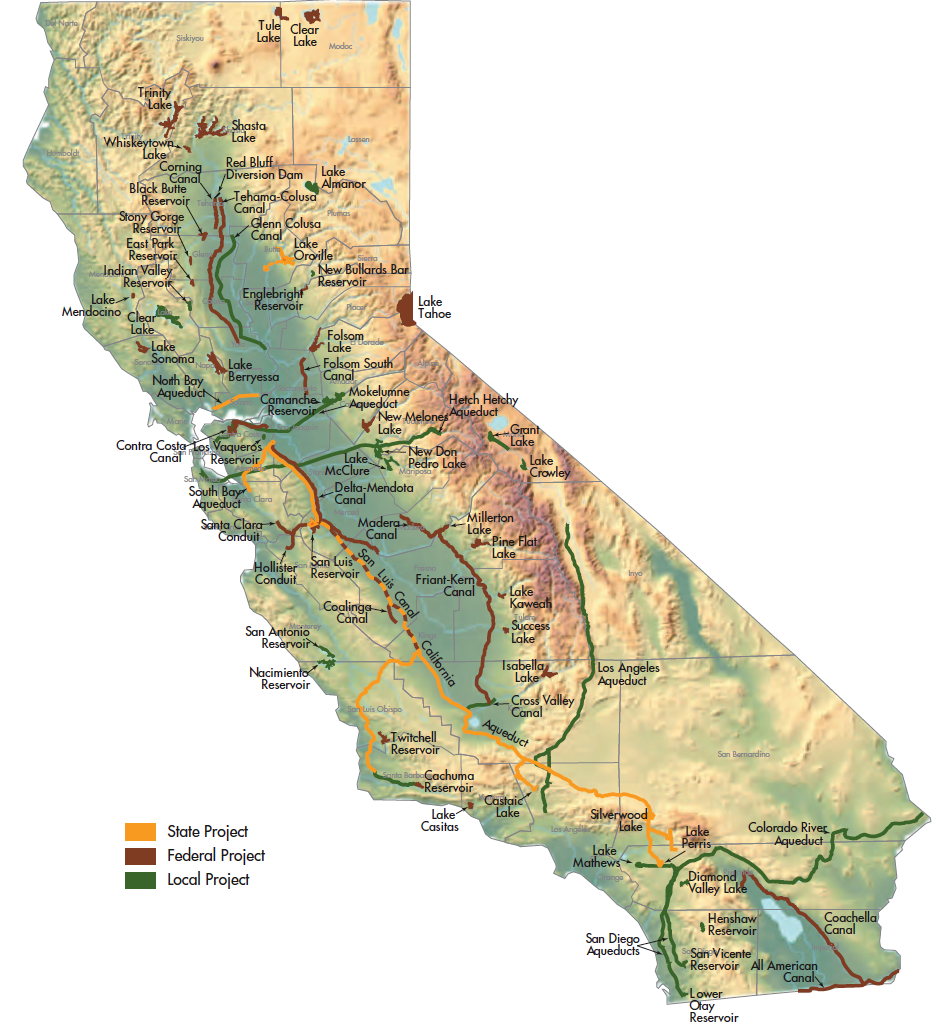
\includegraphics[width=5.5in]{figures/infrastructure.png}
       \caption[Characteristics of Water Distribution Infrastructure]{The geographic extent of water distribution infrastructure in the state of California}
       \label{fig:infrastructure-energy-intensity}
     \end{figure}
    
     \begin{figure}[The energy intensity of water distribution infrastructure in the state California]
       \centering
       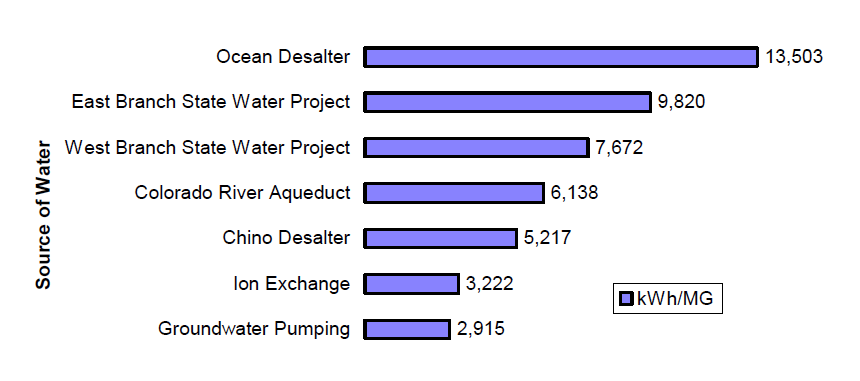
\includegraphics[width=5.5in]{figures/energy-intensity.png}
       \caption[Energy Intensity of Water Distribution Infrastructure]{The geographic extent of water distribution infrastructure in the state California}
       \label{fig:infrastructure-energy-intensity}
     \end{figure}
    
\section{Wastewater Recycling and Reuse}
    
The fastest growing source of new water supply in the state of California is treated wastewater. A major driver behind this trend has been the fact that treated wastewater can be a energy efficient water supply option for a number of low quality uses, particularly when the end-use location is situated in close proximity to the wastewater treatment plant (WWTP). An illustrative example of such a condition might be the use of wastewater which had been subjected to basic secondary treatment for the irrigation of a nearby cemetery or golf course within an urban area.
    
     \begin{figure}[Process flow diagram of various wastewater treatment methods]
       \centering
       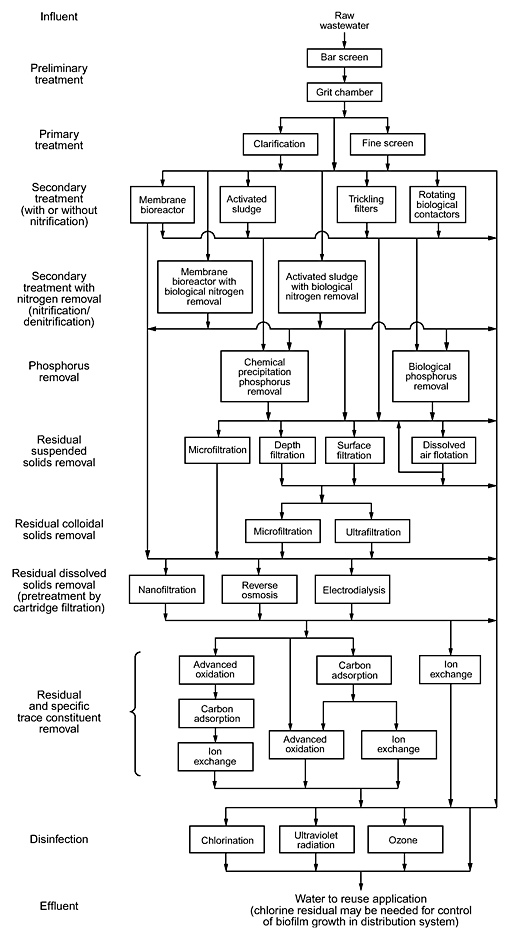
\includegraphics[width=3in]{figures/process-flow.png}
       \caption[Process Flow Diagram of Wastewater Treatment Methods]{Process flow diagram of various wastewater treatment methods}
       \label{fig:process-flow-diagram}
     \end{figure}
    
The term "wastewater treatment" refers to a process of removing physical, chemical, or biological contaminants from a quantity of water such that their concentrations are sufficiently low for that quantity of water to be deemed fit for use in some specified application. Crucially implicit in this definition therefore, is the notion that the treatment methods, and any associated support systems involved, will vary on the basis of the purity requirements associated with the anticipated water end-use type. Figure provides a process flow diagram which demonstrates, in generic terms, the various phases of wastewater treatment and some of the methods/systems that are commonly used at each phase. Adjacent to this, on the right, is a list of common water end use types organized on the basis of the minimum degree of required pretreatment.
    
     \begin{figure}[End Use Categories for Recycled Water]
       \centering
       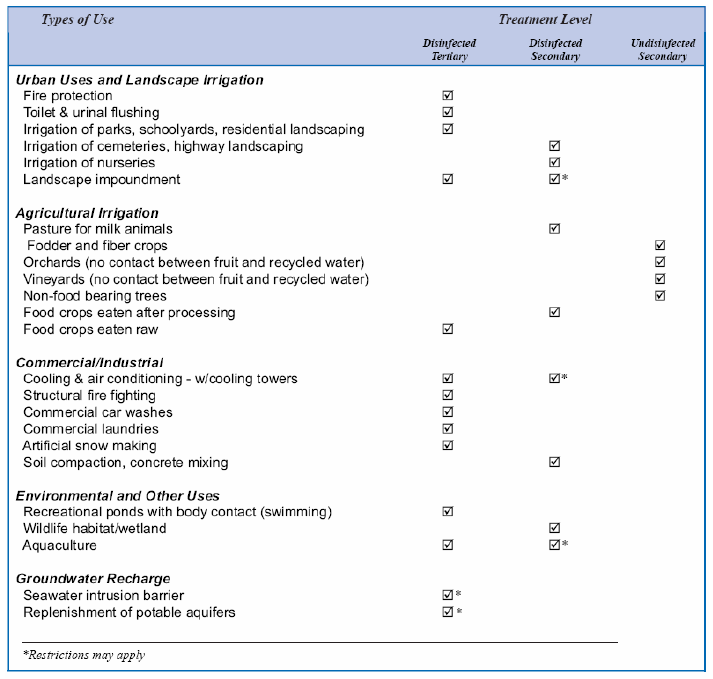
\includegraphics[width=5.5in]{figures/use-categories.png}
       \caption[End Use Categories for Recycled Water]{End Use Categories for Recycled Water}
       \label{fig:use-categories}
     \end{figure}        
              
 \section{Quantifying Life Cycle Energy Usage}

